\documentclass[phd,tocprelim]{cornell}
\usepackage{graphicx,pstricks}
\usepackage{graphics}
\usepackage{subfigure}
\usepackage{epsfig}
\usepackage{subfigure}
\usepackage{hangcaption}
\usepackage{palatino}
\usepackage{natbib}
\usepackage[hidelinks]{hyperref}
\usepackage{color}
\usepackage{amsmath,amsthm,verbatim,amssymb,amsfonts,amscd,mathrsfs}
\usepackage[algo2e,ruled]{algorithm2e}
\usepackage{booktabs} % for professional tables
\usepackage{multirow}
\usepackage{makecell}  % thead, other vertical alignment options
\usepackage{hhline}  % double horizontal lines for tables


%%%%%%%%%%%%%% Custom comments stuff
\newif\ifcomments
%\commentsfalse
\commentstrue
\ifcomments\newcommand{\comments}[1]{#1}\else\newcommand{\comments}[1]{}\fi
\definecolor{clrgp}{rgb}{.9,0,.9}
\newcommand{\gp}[1]{\comments{\textcolor{clrgp}{[GP: #1]}}}


%%%%%%%%%%%%%% Formatting
\bibliographystyle{plainnat}
\renewcommand{\cite}[1]{\citep{#1}}
\renewcommand{\caption}[1]{\singlespacing\hangcaption{#1}\normalspacing}
\renewcommand{\topfraction}{0.85}
\renewcommand{\textfraction}{0.1}
\renewcommand{\floatpagefraction}{0.75}
%if you're having problems with overfull boxes, you may need to increase
%the tolerance to 9999
\tolerance=9999


%%%%%%%%%%%%%%%%%%%%%%%%%%%
\title{Uncertainty Estimations for Modern Machine Learning Algorithms}
\author{Geoff Pleiss}
\conferraldate{May}{2020}
\degreefield{Ph.D.}
\copyrightholder{Geoff Pleiss}
\copyrightyear{2020}


%%%%%%%%%%%%%%%%%%%%%%%%%%%
\begin{document}
\maketitle
\makecopyright

\begin{abstract}
  Gaussian processes (GPs) exhibit a classic tension of many machine learning methods:
they possess desirable modelling capabilities yet suffer from important practical limitations.
In many instances, GPs are able to offer well-calibrated uncertainty estimates, interpretable predictions, and the ability to encode prior knowledge.
These properties have made them an indispensable tool for black-box optimization, time series forecasting, and high-risk applications like health care.
Despite these benefits, GPs are typically not applied to datasets with more than a few thousand data points.
This is in part due to an inference procedure that requires matrix inverses, determinants, and other expensive operations.
Moreover, specialty models often require significant implementation efforts.

This thesis aims to alleviate these practical concerns through a single simple design decision.
Taking inspiration from neural network libraries, we construct GP inference algorithms using only \emph{matrix-vector multiplications} (MVMs) and other linear operations.
This MVM-based approach simultaneously address several of these practical concerns: it reduces asymptotic complexity, effectively utilizes GPU hardware, and provides straight-forward implementations for many specialty GP models.

The chapters of this thesis each address a different aspect of Gaussian process inference.
\cref{chapter:bbmm} introduces a MVM method for training Gaussian process regression models (i.e. optimizing kernel/likelihood hyperparameters).
This approach unifies several existing methods into a highly-parallel and stable algorithm.
\cref{chapter:love} focuses on making predictions with Gaussian processes.
A memory-efficient cache, which can be computed through MVMs, significantly reduces the computation of predictive distributions.
\cref{chapter:ciq} introduces a multi-purpose MVM algorithm that can be used to draw samples from GP posteriors and perform approximate Gaussian process inference.
All three of these methods offer speedups ranging from $4\times$ to $40\times$.
Importantly, applying any of these algorithms to specialty models (e.g. multitask GPs and scalable approximations) simply requires a matrix-vector multiplication routine that exploits covariance structure afforded by the model.

The MVM methods from this thesis form the building blocks of the \href{http://github.com/cornellius-gp/gpytorch}{\tt GPyTorch} library, an open-sourced GP implementation designed for scalability and simple implementations.
In the final chapter, we evaluate GPyTorch models on several large-scale regression datasets.
Using the proposed MVM methods, we can apply exact Gaussian processes to datasets that are \emph{2 orders of magnitude larger} than what has previously been reported---up to 1 million data points.

\end{abstract}

\begin{biosketch}
  Geoff Pleiss was born and raised in the Bay Area, though his journey into machine learning did not begin until his senior year of college.
He graduated from Olin College of Engineering in 2013 with a self-designed engineering degree, specializing in applied math and computing.
After a brief stint as a software developer and consultant at Pivotal Labs in New York City, Geoff moved to Ithaca where he began his PhD work.
At Cornell, Geoff studied machine learning under the advising of Kilian Q. Weinberger.
He is currently a researcher as ASAPP Inc.

%In west Philadelphia born and raised on the playground was where I spent most of my days.
%Chillin' out maxin' relaxin' all cool and all shootin some b-ball outside of the school,
%when a couple of guys who were up to no good started making trouble in my neighborhood.
%I got in one little fight and my mom got scared.
%She said ``You're movin' with your auntie and uncle in Bel Air.''
%I begged and pleaded with her day after day but she packed my suit case and sent me on my way.
%She gave me a kiss and then she gave me my ticket.
%I put my Walkman on and said, ``I might as well kick it.''
%First class, yo this is bad---drinking orange juice out of a champagne glass.
%Is this what the people of Bel-Air living like?
%Hmm this might be alright.
%But wait I hear they're prissy, bourgeois, all that---is this the type of place that they just send this cool cat?
%I don't think so; I'll see when I get there.
%I hope they're prepared for the prince of Bel-Air.
%Well, the plane landed and when I came out there was a dude who looked like a cop standing there with my name out.
%I ain't trying to get arrested yet.
%I just got here.
%I sprang with the quickness like lightning, disappeared.
%I whistled for a cab and when it came near the license plate said fresh and it had dice in the mirror.
%If anything I could say that this cab was rare, but I thought ``Nah, forget it---Yo, homes to Bel Air.''
%I pulled up to the house about seven or eight, and I yelled to the cabbie, ``Yo homes smell ya later!''
%I looked at my kingdom; I was finally there to sit on my throne as the Prince of Bel Air.

\end{biosketch}

\begin{dedication}
  This thesis is dedicated to my parents, Mike and Chris Pleiss, who have always been my role models in science.
I cannot thank you enough for all of your love, encouragement, and support over the years.

\end{dedication}

\begin{acknowledgements}
  Your acknowledgements go here. Make sure it sits inside the brackets.

\end{acknowledgements}

\contentspage
\tablelistpage
\figurelistpage
\normalspacing \setcounter{page}{1} \pagenumbering{arabic}
\pagestyle{cornell} \addtolength{\parskip}{0.5\baselineskip}
\DeclareMathOperator*{\argmax}{arg\,max}
\DeclareMathOperator*{\argmin}{arg\,min}
\DeclareMathOperator*{\expectedvalue}{\mathbb{E}}
\DeclareMathOperator*{\variance}{Var}
\DeclareMathOperator*{\covariance}{Cov}
\DeclareMathOperator*{\trace}{Tr}

% Probability
\newcommand{\bigo}[1]{\ensuremath{\mathchoice{\mathcal O \! \left( #1 \right)}}{\mathcal O ( #1 )}{}{}}
\newcommand{\bigomega}[1]{\ensuremath{\mathchoice{\Omega \! \left( #1 \right)}}{\Omega ( #1 )}{}{}}
\newcommand{\ints}{\ensuremath{\mathbb{Z}}}
\newcommand{\reals}{\ensuremath{\mathbb{R}}}
\newcommand{\GP}[2]{\ensuremath{\mathcal{GP} \left[ #1, #2 \right]}}
\newcommand{\normaldist}[2]{\ensuremath{\mathcal{N} \left[ #1, #2 \right]}}
\renewcommand{\Pr}[1]{\ensuremath{\text{Pr} \left[ #1 \right]}}
\newcommand{\Ev}[1]{\ensuremath{\expectedvalue \left[ #1 \right]}}
\newcommand{\Evover}[2]{\ensuremath{\expectedvalue_{#1} \left[ #2 \right]}}
\newcommand{\Var}[1]{\ensuremath{\variance \left[ #1 \right]}}
\newcommand{\Varover}[2]{\ensuremath{\variance_{#1} \left[ #2 \right]}}
\newcommand{\Cov}[1]{\ensuremath{\covariance \left[ #1 \right]}}
\newcommand{\Covover}[2]{\ensuremath{\covariance_{#1} \left[ #2 \right]}}
\newcommand{\given}{\mid}

% Other matrix/math operators
\newcommand{\tr}[1]{\ensuremath{\mathchoice{\trace \left( #1 \right)}{\trace ( #1 )}{}{}}}
\newcommand{\inv}{^{-1}}
\newcommand{\trans}{^{\top}}
\newcommand{\intd}[1]{\,\mathrm{d}{#1}}

% Matrices / vectors
\newif\ifboldmatrix
\boldmatrixtrue
\ifboldmatrix\newcommand{\boldmatrix}[1]{\mathbf{#1}}\else\newcommand{\boldmatrix}[1]{#1}\fi
\newcommand{\ba}{\ensuremath{\mathbf{a}}}
\newcommand{\bb}{\ensuremath{\mathbf{b}}}
\newcommand{\bd}{\ensuremath{\mathbf{d}}}
\newcommand{\be}{\ensuremath{\mathbf{e}}}
\newcommand{\bfn}{\ensuremath{\mathbf{f}}}
\newcommand{\bk}{\ensuremath{\mathbf{k}}}
\newcommand{\bm}{\ensuremath{\mathbf{m}}}
\newcommand{\bmu}{\ensuremath{\boldsymbol{\mu}}}
\newcommand{\bp}{\ensuremath{\mathbf{p}}}
\newcommand{\bq}{\ensuremath{\mathbf{q}}}
\newcommand{\br}{\ensuremath{\mathbf{r}}}
\newcommand{\bs}{\ensuremath{\mathbf{s}}}
\newcommand{\bt}{\ensuremath{\mathbf{t}}}
\newcommand{\btheta}{\ensuremath{\boldsymbol{\theta}}}
\newcommand{\bu}{\ensuremath{\mathbf{u}}}
\newcommand{\bv}{\ensuremath{\mathbf{v}}}
\newcommand{\bw}{\ensuremath{\mathbf{w}}}
\newcommand{\bx}{\ensuremath{\mathbf{x}}}
\newcommand{\by}{\ensuremath{\mathbf{y}}}
\newcommand{\bz}{\ensuremath{\mathbf{z}}}
\newcommand{\bzero}{\ensuremath{\mathbf{0}}}
\newcommand{\bone}{\ensuremath{\mathbf{1}}}
\newcommand{\bA}{\ensuremath{\boldmatrix{A}}}
\newcommand{\bB}{\ensuremath{\boldmatrix{B}}}
\newcommand{\bC}{\ensuremath{\boldmatrix{C}}}
\newcommand{\bD}{\ensuremath{\boldmatrix{D}}}
\newcommand{\bI}{\ensuremath{\boldmatrix{I}}}
\newcommand{\bK}{\ensuremath{\boldmatrix{K}}}
\newcommand{\bL}{\ensuremath{\boldmatrix{L}}}
\newcommand{\bM}{\ensuremath{\boldmatrix{M}}}
\newcommand{\bP}{\ensuremath{\boldmatrix{P}}}
\newcommand{\bQ}{\ensuremath{\boldmatrix{Q}}}
\newcommand{\bR}{\ensuremath{\boldmatrix{R}}}
\newcommand{\bSigma}{\ensuremath{\boldsymbol{\Sigma}}}
\newcommand{\bT}{\ensuremath{\boldmatrix{T}}}
\newcommand{\bU}{\ensuremath{\boldmatrix{U}}}
\newcommand{\bV}{\ensuremath{\boldmatrix{V}}}
\newcommand{\bW}{\ensuremath{\boldmatrix{W}}}
\newcommand{\bX}{\ensuremath{\boldmatrix{X}}}
\newcommand{\bY}{\ensuremath{\boldmatrix{Y}}}
\newcommand{\bZ}{\ensuremath{\boldmatrix{Z}}}

% Constants
\newcommand{\numdata}{\ensuremath{N}}
\newcommand{\numdim}{\ensuremath{D}}
\newcommand{\numinduc}{\ensuremath{M}}

% Data/dataset specific terms
\newcommand{\bxtest}{\ensuremath{\bx^*}}
\newcommand{\bxtestprime}{\ensuremath{\bx^{*\prime}}}
\newcommand{\bXtest}{\ensuremath{\bX^*}}
\newcommand{\ytest}{\ensuremath{y^*}}
\newcommand{\ytestprime}{\ensuremath{y^{*\prime}}}
\newcommand{\bytest}{\ensuremath{\by^*}}
\newcommand{\meantest}[1]{\ensuremath{\mu^* \left( #1 \right)}}
\newcommand{\bmeantest}[1]{\ensuremath{\bmu^* \left( #1 \right)}}
\newcommand{\covtest}[1]{\ensuremath{\sigma^* \left( #1 \right)}}
\newcommand{\Covtest}[1]{\ensuremath{\bSigma^* \left( #1 \right)}}
\newcommand{\dset}{\ensuremath{\mathcal D}}
\newcommand{\model}{\ensuremath{\mathcal M}}
\newcommand{\loglik}{\ensuremath{\mathcal L}}
\newcommand{\approxK}{\ensuremath{\widetilde{\bK}_{\bX\bX}}}
\newcommand{\trainK}{\ensuremath{\widehat{\bK}_{\bX\bX}}}
\newcommand{\trainP}{\ensuremath{\widehat{\bP}}}

% Method specific terms
\newcommand{\mmm}[1]{\ensuremath{\Xi (#1)}}
\newcommand{\mvm}[1]{\ensuremath{\xi ( #1 )}}
\newcommand{\row}[1]{\ensuremath{\rho ( #1 )}}


\chapter{Introduction}
\label{chapter:introduction}

%Machine learning hype <- success in many different areas.
%Success in many different areas <- advances in algorithms.
%Advances of algorithms <- both in terms of raw potential and in terms of the practical.
%The best algorithms are ones that offer both potential and practicality.
%No one algorithm is perfect <- we need a quiver of different possible algorithms.

%Don't talk about advances.
%Find a lead in to discuss algorithms.

%At this point in machine learning we have several sets of algorithms.

%Questions we need to answer:
%- Why is it important to have multiple algorithms?
%- What kind of algorithms are we looking for?

%Of course, no one algorithm is good at every possible task.
%For example, on many computer vision tasks it is commonly assumed there will be some sort of convolutional layers.
%On many Kaggle competitions, a majority of winning submissions utilize random forests.
%Therefore, it is arguably good to have a variety of possible algorithms.



%Neural networks.

The past decade has witnessed a wide-scale adoption of machine learning methods across numerous application domains.
%Here we will highlight two broad categories of methodological innovation that have contributed to this surge.
This surge is due to the confluence of several factors, of which we will highlight two.
First, researchers have demonstrated the unparalleled {\bf predictive capabilities} of several machine learning algorithms.
%Models can achieve superhuman performance on complex tasks like object recognition \cite{he2016deep}, machine translation \cite{vaswani2017attention}, and strategy game-playing \cite{silver2017mastering}.
At the same time, the community has developed algorithms that are increasingly {\bf practical and easy-to-use}.
Many models can be trained rapidly on consumer-level computer hardware \cite{howard2018training}, and high-quality software frameworks enable practitioners to rapidly develop new models.
%While many other factors have contributed to the machine learning surge, we will limit our focus to these two categories.
While machine learning's predictive successes have opened up new possibilities, its new-found ease-of-use has accelerated innovation and adoption.

Arguably, the machine learning algorithms which have had the broadest impact are the ones that seamlessly offer \emph{both} predictive power and practicality.
Deep neural networks perhaps best exemplify this trend.
Recent innovations in
network architecture \citep[e.g.][]{he2016deep,vaswani2017attention,devlin2018bert,huang2019convolutional},
optimization \citep[e.g.][]{ioffe2015batch,izmailov2018averaging},
and theoretical understanding \citep[e.g.][]{keskar2016large,jacot2018neural,arora2019fine}
have led to massive performance improvements on increasingly complex datasets.
Moreover, these innovations have been complemented by
the effective use of specialty compute hardware (such as GPUs and TPUs),
the introduction of automatic differentiation \citep[e.g.][]{paszke2017automatic},
and the development of of several high-quality software implementations~\citep[e.g.][]{jia2014caffe,abadi2016tensorflow,paszke2019pytorch}.
These pragmatic advances make it easy for practitioners to experiment with new models and architectures, which has undoubtedly contributed to its profound and wide-spread successes \cite{goodfellow2016deep}.

Gradient-boosted trees have a similar powerful-yet-practical story.
Since their inception \cite{friedman2001greedy,friedman2002stochastic}, gradient boosted trees have excelled in many applications \citep[e.g.][]{richardson2007predicting,burges2010ranknet}.
The predictive power of these models is a product of several key attributes: for example, their remarkable generalization properties \citep{freund1997decision,schapire2013boosting} and their ability to handle incomplete features \cite{friedman2001greedy}.
Equally important, these models are simple and computational efficient, in large part due to specialty parallel algorithms \citep[e.g.][]{tyree2011parallel,ke2017lightgbm} and easy-to-use software implementations such as XGBoost \cite{chen2016xgboost}.
These advantages have made gradient-boosted decision trees a workhorse algorithm for many practitioners across application domains.
According to a survey collected by \citet{kaggle2019kaggle}, $75\%$ of the responding data scientists regularly use gradient-boosted decision trees and the XGBoost software.

Nevertheless, for many machine learning algorithms there is still a trade-off between predictive potential and practical limitations.
The focus of this thesis is {\bf Gaussian process models} (GPs), which perhaps best exemplify this tension.
Within the machine learning community, GPs have been well-regarded as a powerful model class with many desirable properties---such as calibrated uncertainty estimates and interpretable model priors.
Recent work on hierarchical modelling \citep[e.g.][]{damianou2013deep} and scalability \citep[e.g.][]{wilson2015kernel} have furthered their applicability to increasingly complex tasks.
However, Gaussian processes have historically been relegated to small datasets, and the tools most commonly used for inference do not effectively utilize modern compute hardware.
%Scalable approximations can remedy these concerns to some extent, yet such approximations can sometimes bias the model's predictions \cite{turner2011two,bauer2016understanding}.
%Finally, new
Using GPs requires significant implementation effort, as simple modifications like an additional output dimension might require different learning/inference procedures.
These practical considerations hinder the adoption of GPs, while also limiting researchers' abilities to rapidly-prototype and make new developments.
This thesis aims to address these limitations so that Gaussian processes can be powerful-\emph{and}-practical models.

% Even as Moore's law runs out, specialty hardware

\section{The Predictive Power of Gaussian Processes Models}

Before addressing these issues, it is worth discussing why Gaussian processes are an invaluable model class for blackbox optimization \citep[e.g.][]{snoek2012practical}, robotics \citep[e.g.][]{deisenroth2011pilco}, health care \citep[e.g.][]{schulam2015framework}, and many other domains:
\begin{enumerate}
  \item {\bf Closed-form marginalization over hypotheses.}
    Many machine learning algorithms (such as neural networks) construct a single model by optimizing over thousands or millions of parameters.
    Gaussian processes on the other hand marginalize over all possible predictive models $f(\cdot)$:
    \[
      p_\text{GP} ( y \mid \bx ) = \int_{f(\cdot)} p( y \mid \bx, f(\cdot)) \: p(f(\cdot)) \: \intd f(\cdot).
    \]
    As a result, the predictions are less prone to overfitting \cite{rasmussen2006gaussian}.

  \item {\bf Well-calibrated uncertainty estimates.}
    The output of a Gaussian process is a predictive \emph{distribution}, which incorporates both modelling uncertainty (e.g. how many different models could fit the data) and data uncertainty (e.g. how noisy are the training data).
    Consequentially, the predictive uncertainties tend to be very well calibrated to the data distribution.

  \item {\bf A flexible language for encoding prior knowledge.}
    A Gaussian process' generalization capabilities are almost entirely determined by its modelling priors.
    Crucially, GP priors directly encode functional properties---such as smoothness, periodicity, or monotonicity---rather than beliefs about certain parameters.
    These functional properties are determined by the choice of \emph{kernel function}, which can be easily composed (see \cref{sec:common_kernels}).
    With the appropriate choice of prior, it is possible to generalize on datasets with as few as 10 observations \citep[e.g.][]{rasmussen2006gaussian,gardner2017discovering}.
    %Several recent works have simplified the task of constructing appropriate kernels, either through composition \citep{duvenaud2013structure} or through differentiable learning \citep{wilson2013gaussian}.

  \item {\bf Interpretable predictions.}
    The predictions from Gaussian processes (see \cref{eqn:predictive_mean,eqn:predictive_var}) are not only expressive and powerful; they are also very intuitive.
    If we view the GP's kernel function as a similarity/distance measure between two points, then the prediction at a given point $\bx$ is simply an interpolation of nearby training points.
    The prediction's confidence interval is small when $\bx$ is close to training points, and large when $\bx$ is too far away for accurate interpolation.
\end{enumerate}
%
\noindent
These benefits are obviously applicable in the ``small data'' regime, where priors and marginalization are critical for meaningful predictive performance \cite{rasmussen2001occam}.
However, these properties also are beneficial for large datasets.
Good uncertainty estimates and interpretable predictions are increasingly desirable for large-scale machine learning models.
%GPs (with certain kernel functions) are universal approximators \cite{micchelli2006universal}, and their modelling capacity increases with the amount of available training data.
In addition, large datasets make it possible to use powerful families of covariance functions \citep{wilson2013gaussian,wilson2016deep,benton2019function} or hierarchical (``deep'') GP models \cite{wilson2016deep,salimbeni2017doubly,jankowiak2020deep}.
%This makes GPs especially powerful on big-data tasks like large-scale extrapolation \citep[e.g.][]{jankowiak2020parametric} and high-dimensional optimization \citep[e.g.][]{eriksson2019scalable}.


\section{Practical Concerns with Gaussian Processes Models}

While Gaussian processes offer great predictive potential, there are several practical issues that hinder its use, especially on larger and more complex datasets.

\subsection{Computational Complexity and Memory Requirements}
Given $N$ training data points, Gaussian process models na\"{i}vely require $\bigo{N^3}$ computation and $\bigo{N^2}$ storage.
This complexity comes from computing a $N \times N$ covariance matrix of all training data and computing several non-linear operations (see \cref{sec:gp_models}).
Historically, this has limited exact Gaussian process models to datasets with fewer than $1,\!000$ data points \cite{hensman2013gaussian}.

\subsection{Use of Modern Compute Hardware}
It is worth noting that this $\bigo{N^3}$ computational complexity is not necessarily insurmountable given modern computational hardware.
For example, some deep learning models require many more floating point operations (FLOPs) than large-scale GPs.
A 264-layer DenseNet model \cite{huang2017densely}, common on many computer vision tasks, requires $2.4 \times 10^{18}$ FLOPs to train on $1.2$ million images.
This is essentially a cubic computational requirement, and would be wholly impractical if it were not for specialty compute hardware like GPUs.
Such a model would probably require months to train on standard CPUs, yet can be trained on 8 GPUs in a matter of hours \cite{howard2018training}.

Given the effectiveness of GPU acceleration on large neural networks, one might expect similar performance for large-scale Gaussian processes.
Unfortunately, many GP implementations rely on the Cholesky factorization (see \cref{sec:gp_models}), which does not benefit as readily from modern compute hardware.
GPUs are designed for massively-parallelizable operations such as matrix-multiplication (which is the primary numerical operation of neural networks).
A matrix-multiply between two $1,\!000 \times 1,\!000$ matrices is $10,\!000$ times faster on a GPU than on a CPU!\footnote{
	As measured on a NVIDIA GTX 1070 GPU verses an 8-core Intel i7 CPU.
}
%which is why large neural networks are practical to train.
The Cholesky algorithm on the other hand is inherently sequential and affords minimal parallelization;
factorizing a $1,\!000 \times 1,\!000$ matrix is only $10$ times faster on GPU than on CPU.
This is why we cannot expect neural-network-level speedups for Cholesky-based GPs.
Moreover, the Cholesky factorization requires $\bigo{N^2}$ storage.
This amounts to a terabyte of memory for $N=1,\!000,\!000$---well beyond the capacity of most GPU clusters.

\subsection{Choosing Appropriate Approximations}
To reduce the computational and memory burden, researchers have proposed numerous methods that approximate Gaussian processes with simpler models.
Such models employ low-rank or structured approximations of the $N \times N$ matrices (see \cref{sec:approx_gps}).
Numerous advances have made these approximate methods more powerful while retaining manageable asymptotic complexities.

However, choosing a suitable approximation involves many design choices.
All approximate methods introduce hyperparameters that control the speed/accuracy trade-off, while also making assumptions that might not be well suited to certain datasets.
For example, variational approaches \citep[e.g.][]{titsias2009variational,hensman2013gaussian}---which are a popular general-purpose approximation---tend to overestimate the observational noise, leading to worse predictive uncertainties \cite{turner2011two,bauer2016understanding}.
Structured interpolation methods \cite{wilson2015kernel} alleviate these biases, yet tend to be limited to low-dimensional problems.
While some theoretical guarantees can guide these design decisions \cite{burt2019rates}, choosing a good approximate model is ultimately dataset specific and can require expert knowledge.
%Good performance often requires a large hyperparameter sweep and expert knowledge.

\subsection{Implementation and Programmability}
One compelling advantage of neural networks is their modularity.
Creating a novel neural network architecture requires significant thought and experimentation; however, \emph{implementing} new architectures requires very little software engineering effort.
Seemingly complex models like DenseNets \cite{huang2017densely} and Transformers \cite{vaswani2017attention} have surprisingly simple implementations using compositional layers.
Small modifications, such as adding an additional output dimension, often require only a single additional line of code.

Gaussian processes models on the other hand require significant implementation effort.
Often, the \emph{model} and the \emph{learning/inference procedures} are tightly coupled.
As an example, consider a Gaussian process with multiple output dimensions \cite{bonilla2008multi}.
While this model and a standard (single-output) GP are seemingly similar, they require completely different implementations.
The additional output dimension changes the structure of the prior covariance matrix (see \cref{sec:programmability}), modifying the equations used for efficient inference.
In the popular \citet{gpy2014} software package, multi-output GPs and standard GPs are implemented as separate models, with multi-output GPs requiring an additional 100 lines of code.
Compared to the one-line change for multi-output neural networks, GPs are significantly more difficult to implement.



\section{Outline of Contributions}
This thesis introduces a framework that addresses these issues without sacrificing the desirable properties of GPs.
Our approach is centered on a \emph{single} critical design decision:
taking inspiration from neural networks, we build GP training and inference algorithms \emph{using only matrix-multiplication} and element-wise operations.
As we will demonstrate, this reduces the asymptotic complexity of GPs, improves their GPU utilization, expands the applicability of exact methods, and simplifies implementation of specialty models.
The following chapters introduce the components of our matrix-multiplication-based framework:

\begin{itemize}
  \item In {\bf \cref{chapter:bbmm}}, we introduce the {\bf BlackBox~Matrix~$\times$~Matrix~(BBMM)} approach for training Gaussian process regression models.
    BBMM uses a modified version of preconditioned conjugate gradients (mPCG) that reduces GP training to a series of \emph{matrix-multiplications}.
    We demonstrate that this approach effectively uses GPU acceleration and is up to $30\times$ faster than existing training methods.
    Additionally, we show that implementing specialty GP models with BBMM only requires writing an efficient kernel matrix-multiplication routine.

  \item {\bf \cref{chapter:love}} focuses on making predictions with Gaussian processes.
    %Computing GP predictive distributions requires expensive computations involving the training covariance matrix.
    We introduce an algorithm---{\bf LancZos~Variance~Estimates~(LOVE)}---that efficiently pre-computes many of the terms required for predictions.
    As with BBMM training, LOVE relies entirely on \emph{matrix-multiplication}, which is especially beneficial for models with fast kernel routines.
    After a simple precomputation, computing GP predictions is \emph{linear} in the amount of training data, or $\bigo{1}$ time if used in conjunction with structured kernel interpolation \cite{wilson2015kernel}.

  \item {\bf \cref{chapter:ciq}} focuses on Gaussian process models with non-Gaussian likelihood functions---i.e. GPs that are used to model heavy-tailed noise, arrival processes, or classification problems.
    Unlike with GP regression, these models necessitate the use of approximate Bayesian inference methods.
    We introduce a matrix-multiplication method based on {\bf Cauchy Integral Quadrature (CIQ)} which can be used to optimize a re-parameterized variational training objective.
    On several large-scale spatial datasets, CIQ enables faster optimization and higher-fidelity approximations than existing methods.
    We also demonstrate that CIQ can be used to efficiently sample from GP posteriors.

  \item This thesis culminates with with {\bf \cref{chapter:largeexact}}, which utilizes the prior chapter's methods to scale GP regression to extremely large datasets.
    Combining BBMM and LOVE with partitioned matrix-multiplication routines, we demonstrate that Gaussian processes can be trained \emph{without approximation} on datasets with \emph{over 1 million data points}.
    GPU-acceleration makes these large-scale GPs roughly as fast as approximate methods, despite their larger asymptotic complexity.
    We perform the first-ever comparison of exact GPs against scalable approximations on datasets with $10^4$---$10^6$ data points, showing dramatic performance improvements.
\end{itemize}
%
\noindent
Finally, we package together these contributions into {\bf GPyTorch},\footnote{
  \url{http://gpytorch.ai}
}
an open-source implementation of BBMM, LOVE, and CIQ.
GPyTorch can be used to build small-scale or large-scale GPs with flexible neural-network-like building blocks.
Moreover, the package seamlessly integrates with PyTorch \cite{paszke2019pytorch}, Pyro \cite{bingham2019pyro}, and BoTorch \cite{balandat2019botorch} to combine GPs with neural networks, probablistic models, and blackbox optimizers.
Throughout this thesis, we will discuss how the various algorithms (BBMM, LOVE, and CIQ) are implemented in GPyTorch, and how a practitioner can build on top of them to develop novel GP models.

We begin with a brief overview of Gaussian process models, common kernel functions, and scalable GP approximations.
Additionally, we introduce Krylov-subspace methods---a family of numerical algorithms that compute matrix functions through matrix-vector products---which form the foundation of our matrix-multiplication-based GP framework.

% In fact, we are not simply going to take inspiration from Neural networks, we are going to directly exploit those tools

%\paragraph{Preventing catastrophic failure.}

%\paragraph{Improved predictive pipelines.}

%\paragraph{Detecting anomalous inputs.}
%Machine learning models will only generalize to data that are sufficiently similar to the training data.
%If a model encounters \emph{out-of-distribution} (OOD) inputs -- inputs that deviate from the distribution of training data -- its predictions are likely to be erroneous or nonsensical \cite{begoli2019uncertainty,jiang2012calibrating}.
%%This may occur if the model is used in scenarios that experience covariate shift \cite{sugiyama2007covariate} or if the model encounters previously-unseen categories of data \cite{yu2017occ,hassen2018openset}.
%%Such scenarios are examples of \emph{out-of-distribution} (OOD) inputs.
%This phenomenon is illustrated in \cref{fig:ood_teaser}, which displays predictions from a neural network trained to predict prices of middle-class houses in Kentucky.
%The model is able to make sensible predictions on other Kentucky houses (left and center-left images).
%At the same time, the model vastly underestimates the price of a California mansion (center-right) and predicts and absurdly large price for a chair (right), as these inputs are not similar to any of the training set inputs.
%This is because the range of predicted prices for the out-of-distribution matches the range of Kentucky housing prices.
%A practitioner would see that the predictions are well within the model's expected output values and would be unaware that these predictions are nonsensical given the supplied inputs.

%Well-modeled uncertainty estimates can to identify potentially anomalous data and prevent such erroneous predictions.
%In this example, \gp{finish}

%\paragraph{A principled exploration/exploitation tradeoff.}

%\paragraph{Interpretability and trustworthiness.}
%Good uncertainty estimates can provide a valuable extra bit of information to users of machine learning models when predictions may otherwise be difficult to interpret.
%As machine learning algorithms become increasingly complex, they also appear more ``black box'' to users of such systems.
%This presents several challenges, especially for models that are used to aid human decision makers in domains such as medicine, finance, and policy \gp{cite}.

%For such circumstances it is therefore desirable for predictions to be understandable or interpretable \gp{cite LIME, saliency, etc.}.
%There are many definitions for what constitutes a good ``explanation'' of black-box predictions, coming from policy makers \gp{cite gdpr, etc} and the research community \gp{cite} alike.
%Though there are disagreements between these various sources, a well-calibrated uncertainty estimate is typically seen as a bare-minimum requirement for an interpretable prediction \gp{cite}.
%Most humans -- even if they are unable to perform simple inferences \cite{gigerenzer2003simple} -- have natural intuition for interpreting confidence estimates as event-occurrence frequencies \cite{cosmides1996humans,hoffrage1998using}.
%Therefore, well-calibrated confidence estimates from ML models can be easily interpreted by users.
%Moreover, the presence of uncertainty estimates can affect a user's trust in a machine learning model.
%In a study by \citet{zhou2017effects}, humans were asked to plan a budget for construction tasks based on information provided by a machine learning model.
%Some participants received both predictions and confidence intervals from the machine learning model, while other users only received the predictions.
%On tasks with low-to-moderate cognitive overhead, participants who saw uncertainty scores reported higher levels of trust in the machine learning model.

\chapter{Calibrating Neural Network Confidence Estimates for Classification.}
\section{Introduction}
\label{sec:nn-calibration:introduction}

Recent advances in deep learning have dramatically improved neural network accuracy \citep{simonyan2014very, srivastava2015highway, he2015deep, huang2016deep, huang2016densely}.
As a result, neural networks are now entrusted with making complex decisions in applications, such as object detection \cite{girshick2015fast}, speech recognition \cite{hannun2014deep}, and medical diagnosis \cite{caruana2015intelligible}.
In these settings, neural networks are an essential component of larger decision making pipelines.

%In real-world decision making systems, classification networks must not only be accurate, but also should indicate when they are likely to be incorrect.
%As an example, consider a self-driving car that uses a neural network to detect pedestrians and other obstructions \cite{bojarski2016end}.
%If the detection network is not able to confidently predict the presence or absence of immediate obstructions, the car should rely more on the output of other sensors for braking.
%Alternatively, in automated health care, control should be passed on to human doctors when the confidence of a disease diagnosis network is low  \cite{jiang2012calibrating}.
%Specifically, a network should provide a \emph{calibrated confidence} measure in addition to its prediction.
%In other words, the probability associated with the predicted class label should reflect its ground truth correctness likelihood.

\begin{figure}[t!]
  \centering
  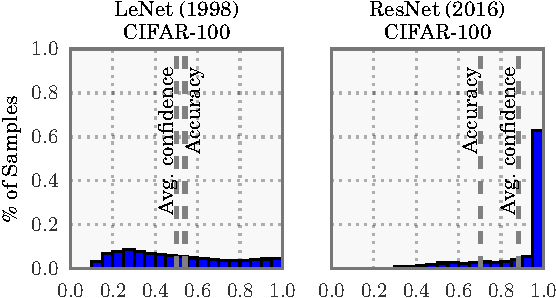
\includegraphics[width=0.8\columnwidth]{figures/confidence.pdf}
  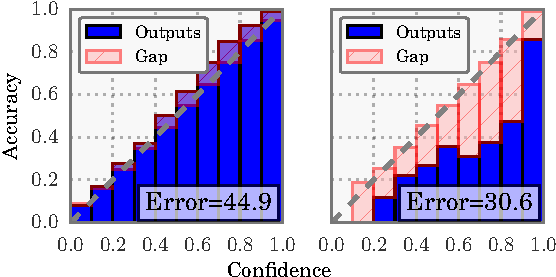
\includegraphics[width=0.8\columnwidth]{figures/comparison_with_caruana.pdf}
  \caption{Confidence histograms (top) and reliability diagrams (bottom) for a 5-layer LeNet (left) and a 110-layer ResNet (right) on CIFAR-100. Refer to the text below for detailed illustration.}
  \label{figure.complenet}
  \vspace{8pt}
\end{figure}

%Calibrated confidence estimates are also important for model interpretability.
%Humans have a natural cognitive intuition for probabilities \cite{cosmides1996humans}.
%Good confidence estimates provide a valuable extra bit of information to establish trustworthiness with the user -- especially for neural networks, whose classification decisions are often difficult to interpret.
Further, good probability estimates can be used to incorporate neural networks into other probabilistic models.
For example, one can improve performance by combining network outputs with a language model in speech recognition \cite{hannun2014deep,xiong2016achieving}, or with camera information for object detection \citep{kendall2015modelling}.

In 2005, \citet{niculescu2005predicting} showed that neural networks typically produce well-calibrated probabilities on binary classification tasks. While neural networks today are undoubtedly more accurate than they were a decade ago,
we discover with great surprise that \emph{modern neural networks are no longer well-calibrated}.
This is visualized in \autoref{figure.complenet}, which compares a 5-layer LeNet (left) \cite{lecun1998gradient} with a 110-layer ResNet (right) \cite{he2015deep} on the CIFAR-100 dataset.
The top row shows the distribution of prediction confidence (i.e. probabilities associated with the predicted label) as histograms.
The average confidence of LeNet closely matches its accuracy, while the average confidence of the ResNet is substantially higher than its accuracy.
% That is, the ResNet is \emph{severely overconfident}.
This is further illustrated in the bottom row reliability diagrams \cite{degroot1983comparison,niculescu2005predicting}, which show accuracy as a function of confidence. We see that LeNet is well-calibrated, as confidence closely approximates the expected accuracy (i.e. the bars align roughly along the diagonal). On the other hand, the ResNet's accuracy is better, but does not match its confidence.

% In this paper, we thoroughly study the problem of calibrating modern neural networks in supervised classification settings.
Our goal is not only to understand why neural networks have become miscalibrated, but also to identify what methods can alleviate this problem.
%
In this paper, we demonstrate on several computer vision and NLP tasks that neural networks produce confidences that do not represent true probabilities.
%
Additionally, we offer insight and intuition into network training and architectural trends that may cause miscalibration.
%
Finally, we compare various post-processing calibration methods on state-of-the-art neural networks, and introduce several extensions of our own. Surprisingly, we find that a single-parameter variant of Platt scaling \cite{platt1999probabilistic} -- which we refer to as \emph{temperature scaling} -- is often the most effective method at obtaining calibrated probabilities. Because this method is straightforward to implement with existing deep learning frameworks, it can be easily adopted in practical settings.
%

%% !TeX root = ../main.tex
\label{sec:definitions}

% reduce display equation skip
 \setlength{\abovedisplayskip}{4pt}
 \setlength{\belowdisplayskip}{4pt}
 \setlength{\textfloatsep}{4pt}

\begin{figure*}[t!]
  \centering
  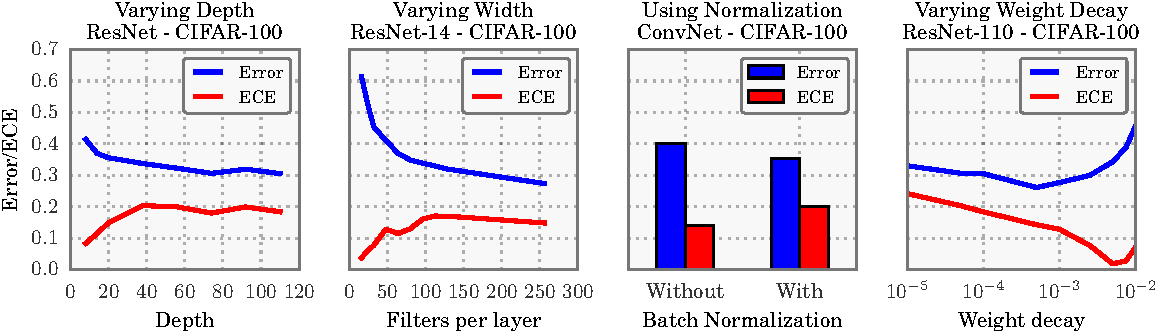
\includegraphics[width=\textwidth]{fig/factors.pdf}
  \caption{The effect of network depth (far left), width (middle left), Batch Normalization (middle right), and weight decay (far right) on miscalibration, as measured by ECE (lower is better).}
  \label{figure.factors}
  \vspace*{-2ex}
\end{figure*}

The problem we address in this paper is supervised multi-class classification with neural networks. The input $X\in\scrX$ and label $Y\in\scrY=\{1, \ldots, K\}$ are random variables that follow a ground truth joint distribution $\pi(X,Y) = \pi(Y|X) \pi(X)$.
Let $h$ be a neural network with $h(X) = (\yh, \ph)$, where $\yh$ is a class prediction and $\ph$ is its associated confidence, i.e. probability of correctness.
We would like the confidence estimate $\ph$ to be calibrated, which intuitively means that $\ph$ represents a true probability. For example, given 100 predictions, each with confidence of $0.8$, we expect that $80$ should be correctly classified.
More formally, we define \emph{perfect calibration} as
\begin{equation}
\label{perfect_calibration}
\P \left(\yh=Y\sep \ph = p\right)=p,\quad\forall p \in [0,1]
\end{equation}
where the probability is over the joint distribution.
%In the Appendix we show that if $h$ recovers the confidence of the ground truth conditional distribution, then $h$ is perfectly calibrated, which justifies this definition.
% \gp{Should we make $X$, $Y$, and $P$ lowercase?}
In all practical settings, achieving perfect calibration is impossible.
Additionally, the probability in \eqref{perfect_calibration} cannot be computed using finitely many samples since $\ph$ is a continuous random variable. This motivates the need for empirical approximations that capture the essence of \eqref{perfect_calibration}.

\paragraph{Reliability Diagrams} (e.g. \autoref{figure.complenet} bottom)
are a visual representation of model calibration \citep{degroot1983comparison,niculescu2005predicting}.
These diagrams plot expected sample accuracy as a function of confidence.
If the model is perfectly calibrated -- i.e. if \eqref{perfect_calibration} holds -- then the diagram should plot the identity function. Any deviation from a perfect diagonal represents miscalibration.

To estimate the expected accuracy from finite samples, we group predictions into $M$ interval bins (each of size $1/M$) and calculate the accuracy of each bin.
Let $B_m$ be the set of indices of samples whose prediction confidence falls into the interval $I_m = (\frac{m-1}{M},\frac{m}{M}]$.
% For samples $x_1,\ldots,x_n$, let $(\hat{y}_i,\hat{p}_i) = h(x_i)$ be the model's predictions and confidence scores for $i = 1,\ldots,n$.
% Let $M$ denote the number of bins, sometimes called the resolution \citep{stefanoonline}. We partition the interval $[0,1]$ into $M$ disjoint intervals $I_m = (\frac{m-1}{M},\frac{m}{M}]$ and define $B_m = \{ i \sep \hat{p}_i \in I_m \}$ for $m = 1,\ldots,M$. A reliability diagram (e.g., \autoref{figure.complenet}) draws bars over each interval $I_m$ whose height corresponds to the average accuracy within that bin, which we denote by
The accuracy of $B_m$ is
%
$$\acc(B_m) = \frac{1}{|B_m|}\sum_{i \in B_m}\ind(\hat{y}_i = y_i),$$
%
where $\hat{y}_i$ and $y_i$ are the predicted and true class labels for
sample $i$.
%
Basic probability tells us that $\acc(B_m)$ is an unbiased and consistent estimator of $\P(\yh = Y \mid \ph \in I_m)$. We define the average confidence within bin $B_m$ as
%
$$\conf(B_m) = \frac{1}{|B_m|}\sum_{i \in B_m}\hat{p}_i,$$
%
where $\hat{p}_i$ is the confidence for sample $i$.
%
$\acc(B_m)$ and $\conf(B_m)$ approximate the left-hand and right-hand sides of \eqref{perfect_calibration} respectively for bin $B_m$.
Therefore, a perfectly calibrated model will have $\acc(B_m) = \conf(B_m)$ for all $m \in \{ 1, \ldots, M \}$.
% As $M \! \rightarrow \! \infty$, we recover the exact definition given by \eqref{perfect_calibration}.
Note that reliability diagrams do not display the proportion of samples in a given bin, and thus cannot be used to estimate how many samples are calibrated.


\paragraph{Expected Calibration Error (ECE).}
While reliability diagrams are useful visual tools, it is more convenient to have a scalar summary statistic of calibration.
Since statistics comparing two distributions cannot be comprehensive, previous works have proposed variants, each with a unique emphasis.
One notion of miscalibration is the difference in expectation between confidence and accuracy, i.e.
%
\begin{align}
  \E_{\ph} \left[ \left| \P\left(\yh = Y \sep \ph = p\right) - p \right| \right]
  \label{eqn:miscalibration}
\end{align}
%
Expected Calibration Error \citep{naeini2015obtaining} -- or ECE -- approximates \eqref{eqn:miscalibration} by partitioning predictions into $M$ equally-spaced bins (similar to the reliability diagrams) and taking a weighted average of the bins' accuracy/confidence difference. More precisely,
\begin{equation}
\label{ece}
\text{ECE} = \sum_{m=1}^{M}\frac{|B_m|}{n}\bigg|\acc(B_m) - \conf(B_m)\bigg|,
\end{equation}
where $n$ is the number of samples.
The difference between $\acc$ and $\conf$ for a given bin represents the calibration \emph{gap} (red bars in reliability diagrams -- e.g. \autoref{figure.complenet}).
%\gp{I think we need to drive home here how to interpret ECE, since we're showing it in many graphs. We need to hammer home that it approximates our probabilistic error.}
We use ECE as the primary empirical metric to measure calibration.
See \autoref{sup:definitions} for more analysis of this metric.
%\cg{Need to rewrite this part...} For each term in the sum, $\text{acc}(B_m) \frac{|B_m|}{n}$ is its {\color{red} unbiased and consistent estimator}. On the RHS, we have $\E_{X}[\ph] = \sum_{m=1}^{M}\E_{X\in B_m}[\ph]$. And for each term in the sum, $\frac{|B_m|}{n}\hat{p}(B_m)$ is an {\color{red} unbiased and consistent estimator}. Together, we obtain an {\color{red} unbiased and consistent estimator} of
%$\E \bigg|\P\left(\yh=Y\sep \ph = p\right)-p\bigg|$.

%Alternatively,
%we know that
%$$ \P\left(Y = \yh\sep \ph\right) = \E_{X,Y} \left[\ind_{Y}(\yh)\sep \ph\right]$$
%and
%$$
%\E\left[ \E_{X,Y} \left[\ind_{Y}(\yh)\sep \ph\right]\right]
%=  \E_{X,Y} \left[\ind_{Y}(\yh)\right] = \P(\yh=Y)
%$$

\paragraph{Maximum Calibration Error (MCE).} In high-risk applications where reliable confidence measures are absolutely necessary, we may wish to minimize the worst-case deviation between confidence and accuracy:
%
\begin{equation}
  \max_{p \in [0, 1]} \left| \P\left(\yh = Y \sep \ph = p\right) - p \right|.
\end{equation}
%
The Maximum Calibration Error \citep{naeini2015obtaining} -- or MCE -- estimates this deviation. Similarly to ECE, this approximation involves binning:
\begin{equation}
\label{mce}
\text{MCE} = \max_{m \in \{1,\ldots,M\} }\left|\acc(B_m) - \conf(B_m)\right|.
\end{equation}
% Thus MCE is an empirical upper bound estimate of $|\P(\yh=Y\sep \ph = p)-p|$.
We can visualize MCE and ECE on reliability diagrams.
MCE is the largest calibration gap (red bars) across all bins, whereas ECE is a weighted average of all gaps.
For perfectly calibrated classifiers, MCE and ECE both equal 0.

\paragraph{Negative log likelihood} is a standard measure of a probabilistic model's quality \cite{friedman2001elements}. It is also referred to as the cross entropy loss in the context of deep learning \cite{bengio2015deep}. Given a probabilistic model $\hat{\pi}(Y|X)$ and $n$ samples, NLL is defined as:
%
\begin{align}
  \scrL = -\sum_{i=1}^{n}\log(\hat{\pi}(y_i|\xb_i))
\end{align}
%
It is a standard result \cite{friedman2001elements} that, in expectation, NLL is minimized if and only if $\hat{\pi}(Y|X)$ recovers the ground truth conditional distribution $\pi(Y|X)$.

%% !TeX root = ../main.tex
% reduce display equation skip
\setlength{\abovedisplayskip}{4pt}
\setlength{\belowdisplayskip}{4pt}
\setlength{\textfloatsep}{4pt}

The architecture and training procedures of neural networks have rapidly evolved in recent years. In this section we identify some recent changes that are responsible for the miscalibration phenomenon observed in \autoref{figure.complenet}.
Though we cannot claim causality, we find that increased model capacity and lack of regularization are closely related to model miscalibration.

% which produces well-calibrated probability scores in traditional settings {\color{red} (cite, cite, cite)}. Indeed, many applications have historically been using these $p_k\in[0,1]$ as actual probabilities \citep{girshick2015fast} {\color{red} (cite)}. In fact, an empirical survey by Niculescu-Mizil and Caruana \citet{niculescu2005predicting} ranked neural networks among the most calibrated models.

% However, a decade has gone by, and as we have already introduced in \autoref{introduction}, deep networks nowadays are poorly calibrated. Following the training recipe exactly as provided by the authors, we observe severe \emph{overconfidence} on various models with state-of-the-art accuracy. In this section we will explore the cause of this phenomenon.
%Here we outline what trends may be causing this miscalibration.
%It'll be important to emphasize that we are not trying to explain why these
%trends cause miscalibration, rather that we are just noticing these trends.

\paragraph{Model capacity.}
The model capacity of neural networks has increased at a dramatic pace over the past few years. It is now common to see networks with hundreds, if not thousands of layers \cite{he2015deep,huang2016deep} and hundreds of convolutional filters per layer \cite{zagoruyko2016wide}. Recent work shows that very deep or wide models are able to generalize better than smaller ones, while exhibiting the capacity to easily fit the training set \cite{zhang2016understanding}.

Although increasing depth and width may reduce classification error, we observe that these increases negatively affect model calibration.
\autoref{figure.factors} displays error and ECE as a function of depth and width on a ResNet trained on CIFAR-100. The far left figure varies depth for a network with 64 convolutional filters per layer, while the middle left figure fixes the depth at 14 layers and varies the number of convolutional filters per layer. Though even the smallest models in the graph exhibit some degree of miscalibration, the ECE metric grows substantially with model capacity.
During training, after the model is able to correctly classify (almost) all training samples, NLL can be further minimized by increasing the confidence of predictions.
Increased model capacity will lower training NLL, and thus the model will be more (over)confident on average.
% We observe that these models also output overly confident probabilities on test samples.
% This trend is also prominent among many other datasets and model architectures.
% Results and figures on the other datasets are included in the supplementary material.

\paragraph{Batch Normalization} \cite{ioffe2015batch} improves the optimization of neural networks by minimizing distribution shifts in activations within the neural network's hidden layers. Recent research suggests that these normalization techniques have enabled the development of very deep architectures, such as ResNets \cite{he2015deep} and DenseNets \cite{huang2016densely}. It has been shown that Batch Normalization improves training time, reduces the need for additional regularization, and can in some cases improve the accuracy of networks.

While it is difficult to pinpoint exactly how Batch Normalization affects the final predictions of a model, we do observe that models trained with Batch Normalization tend to be more miscalibrated. In the middle right plot of \autoref{figure.factors}, we see that a 6-layer ConvNet obtains worse calibration when Batch Normalization is applied, even though classification accuracy improves slightly. We find that this result holds regardless of the hyperparameters used on the Batch Normalization model (i.e. low or high learning rate, etc.).
% It is difficult to attribute the cause of this phenomenon to any particular effect of Batch Normalization.

\begin{figure}[t!]
	\centering
	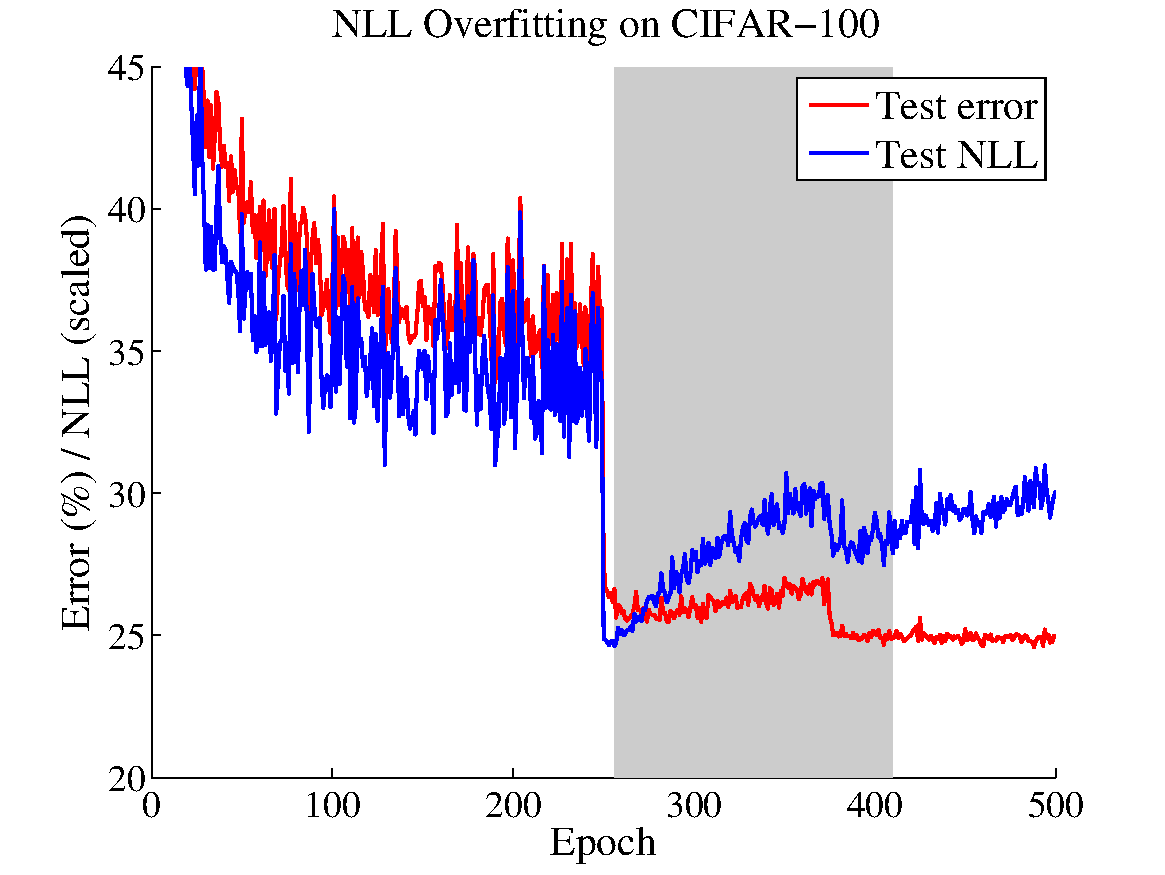
\includegraphics[width=\columnwidth]{fig/cifar100_overfit.pdf}
	\caption{Test error and NLL of a 110-layer ResNet with stochastic depth on CIFAR-100 during training. NLL is scaled by a constant to fit in the figure. Learning rate drops by 10x at epochs 250 and 375. The shaded area marks between epochs at which the best validation \emph{loss} and best validation \emph{error} are produced.}
	\label{figure.cifar100_overfit}
	\vspace{1ex}
\end{figure}

\paragraph{Weight decay,} which used to be the predominant regularization mechanism for neural networks, is decreasingly utilized when training modern neural networks. Learning theory suggests that regularization is necessary to prevent overfitting, especially as model capacity increases \cite{vapnik1998}. However, due to the apparent regularization effects of Batch Normalization, recent research seems to suggest that models with less L2 regularization tend to generalize better \cite{ioffe2015batch}. As a result, it is now common to train models with little weight decay, if any at all. The top performing ImageNet models of 2015 all use an order of magnitude less weight decay than models of previous years \cite{he2015deep, simonyan2014very}.

We find that training with less weight decay has a negative impact on calibration.
The far right plot in \autoref{figure.factors} displays training error and ECE for a 110-layer ResNet with varying amounts of weight decay.
The only other forms of regularization are data augmentation and Batch Normalization.
We observe that calibration and accuracy are not optimized by the same parameter setting.
While the model exhibits both over-regularization and under-regularization with respect to classification error, it does not appear that calibration is negatively impacted by having too much weight decay.
Model calibration continues to improve when more regularization is added, well after the point of achieving optimal accuracy.
The slight uptick at the end of the graph may be an artifact of using a weight decay factor that impedes optimization.

\paragraph{NLL} can be used to indirectly measure model calibration. In practice, we observe \emph{a disconnect between NLL and accuracy}, which may explain the miscalibration in \autoref{figure.factors}.
%
This disconnect occurs because neural networks can \emph{overfit to NLL without overfitting to the 0/1 loss}.
We observe this trend in the training curves of some miscalibrated models.
\autoref{figure.cifar100_overfit} shows test error and NLL (rescaled to match error) on CIFAR-100 as training progresses.
Both error and NLL immediately drop at epoch 250, when the learning rate is dropped; however, NLL overfits during the remainder of training.
Surprisingly, overfitting to NLL is beneficial to classification accuracy. On CIFAR-100, test error drops from $29\%$ to $27\%$ in the region where NLL overfits. This phenomenon renders a concrete explanation of miscalibration: the network learns better classification accuracy at the expense of well-modeled probabilities.

We can connect this finding to recent work examining the generalization of large neural networks. \citet{zhang2016understanding} observe that deep neural networks seemingly violate  the common understanding of learning theory that large models with little regularization will not generalize well. The observed disconnect between NLL and 0/1 loss suggests that these high capacity models are not necessarily immune from overfitting, but rather, overfitting manifests in probabilistic error rather than classification error.
%Though we are not able to explain why this disconnect occurs, it does offer intuition as to why modern neural networks tend to be miscalibrated.

%% !TeX root = ../main.tex
% reduce display equation skip
\setlength{\abovedisplayskip}{4pt}
\setlength{\belowdisplayskip}{4pt}
\setlength{\textfloatsep}{4pt}

In this section, we first review existing calibration methods, and introduce new variants of our own.
%Those methods are comprehensively evaluated in \autoref{results}.
All methods are post-processing steps that produce (calibrated) probabilities.
Each method requires a hold-out validation set, which in practice can be the same set used for hyperparameter tuning.
% Thus calibration does not impose additional training or data collection costs.
We assume that the training, validation, and test sets are drawn from the same distribution.

\subsection{Calibrating Binary Models}
\label{binary_calibration}

We first introduce calibration in the binary setting, i.e. $\mathcal{Y}=\{0,1\}$.
For simplicity, throughout this subsection, we assume the model outputs only the confidence for the positive class.\footnote{
  This is in contrast with the setting in \autoref{definitions}, in which the model produces both a class prediction and confidence.
}
%, i.e. $h(X) = \hat p_i = \P(Y = 1 \sep X)$.
Given a sample $\xb_i$, we have access to $\hat p_i$ -- the network's predicted probability of $y_i = 1$, as well as $z_i \in \mathbb{R}$ -- which is the network's non-probabilistic output, or \emph{logit}. The predicted probability $\hat p_i$ is derived from $z_i$ using a sigmoid function $\sigma$; i.e.
$\hat p_i = \sigma(z_i)$. Our goal is to produce a calibrated probability $\hat q_i$ based on $y_i$, $\hat p_i$, and $z_i$.
% We will use the following notation in this section: for sample $i$, $\xb_i$ is the input features, and $\hat y_i$ and $\hat p_i$ are the predicted class and distribution. Additionally, we assume that we have access to the network's \emph{logit vector} $\zb_i \in \mathbb{R}^K$, which is the output of the final layer before passing through the final softmax function. $\hat y_i$ and $\hat p_i$ can be written in terms of $\zb_i$:
% %
% \begin{align*}
%  \hat y_i &= \argmax_{k \in 1, \ldots, K} \frac{e^{z_i^{(k)}}}{\sum_{j=1}^K e^{z_i^{(j)}}}, \hspace{10pt}
%   \hat p_i = \max_{k \in 1, \ldots, K} \frac{e^{z_i^{(j)}}}{\sum_{j=1}^K e^{z_i^{(j)}}}.
% \end{align*}
% .

\paragraph{Histogram binning} \cite{zadrozny2001obtaining} is a simple non-parametric calibration method.
% Given $n$ samples, let the uncalibrated output probabilities be $\hat{p}_i = h(\xb_i)\in[0,1]$ for samples $i = 1,\ldots,n$.
In a nutshell,  all uncalibrated predictions $\hat{p}_i$ are divided
into mutually exclusive bins $B_1,\dots,B_M$. Each bin is assigned a calibrated score $\theta_m$; i.e. if $\hat p_i$ is assigned to bin $B_m$, then $\hat q_i = \theta_m$. At test time, if prediction $\hat{p}_{te}$ falls into bin $B_m$, then the calibrated prediction $\hat q_{te}$ is $\theta_m$.
%
More precisely, for a suitably chosen $M$ (usually small), we first define bin boundaries $0 = a_1 \leq a_2 \leq \ldots \leq a_{M+1} = 1$, where the bin $B_m$ is defined by the interval $(a_m, a_{m+1}]$.
Typically the bin boundaries are either chosen to be equal length intervals
% (i.e. $a_m = \frac{m-1}{M}$ for all $m$)
or to equalize the number of samples in each bin.
% (i.e. $|B_m| = |B_{m'}|$ for all $m, m'$.)
% The confidence of $B_m$ is the average number of positive class samples in that bin:
% $$\theta_m =  \frac{1}{|B_m|} \sum_{i \in B_m} y_i.$$
The predictions $\theta_i$ are chosen to minimize the bin-wise squared loss:
\begin{equation}
\min_{\theta_1,\ldots,\theta_M} \: \sum_{m=1}^M \sum_{i = 1}^n
\mathbf{1} (a_m \leq \hat p_i < a_{m+1}) \left(\theta_m - y_i \right)^2,
\label{eqn:hist_bin}
\end{equation}
%
where $\mathbf{1}$ is the indicator function. Given fixed bins boundaries, the solution to \eqref{eqn:hist_bin} results in $\theta_m$ that correspond to the average number of positive-class samples in bin $B_m$.

\paragraph{Isotonic regression} \cite{zadrozny2002transforming}, arguably the most common non-parametric calibration method,
learns a piecewise constant function $f$ to transform uncalibrated outputs; i.e. $\hat q_i = f(\hat p_i)$.
Specifically, isotonic regression produces $f$ to minimize the square loss $\sum_{i=1}^n (f(\hat p_i) - y_i)^2$.
Because $f$ is constrained to be piecewise constant, we can write the optimization problem as:
%
\begin{equation}
\begin{aligned}
\label{iso_eq}
% \min_{\substack{M,\theta_1,\ldots,\theta_M \\ a_1,a_2,\ldots,a_{M+1}}} \hspace{4pt} &\sum_{m=1}^M \sum_{\hat{p}_i \in (a_m,a_{m+1}]} (\theta_m - y_i)^2 \\
\min_{\substack{M \\ \theta_1,\ldots,\theta_M \\ a_1,\ldots,a_{M+1}}} & \hspace{3pt} \sum_{m=1}^M \sum_{i = 1}^n
\mathbf{1} (a_m \leq \hat p_i < a_{m+1}) \left(\theta_m - y_i \right)^2 \\
\text{subject to} & \hspace{8pt} 0 = a_1 \leq a_2 \leq \ldots \leq a_{M+1} = 1, \nonumber \\
& \hspace{8pt} \theta_1 \leq \theta_2 \leq \ldots \leq \theta_M. \nonumber
\end{aligned}
\end{equation}
%
where $M$ is the number of intervals; $a_1, \ldots, a_{M+1}$ are the interval boundaries; and $\theta_1, \ldots, \theta_M$ are the function values.
Under this parameterization, isotonic regression is a strict generalization of histogram binning in which the bin boundaries and bin predictions are jointly optimized.

%
% where $i \in B_m$ corresponds to $\hat{p_i} \in (a_m, a_{m+1}]$.
% Similar to histogram binning, the probability for a test point $\xb_{te}$ is given by which bin $\hat{p}_{te}$ falls into.
%
% This method finds a piecewise constant non-decreasing function $f : [0,1] \rightarrow \mathbb{R}$ to transform the uncalibrated predictions; i.e. $\hat q_i = f(p_i)$.
% More specifically, $f$ is chosen to minimizes $\sum_{i=1}^n (f(\hat{p}_i) - y_i)^2.$
% The piecewise intervals of $f$ parameterize the bin endpoints $(a_i, a_{i+1})$ and bin values $\theta_i$.

\paragraph{Bayesian Binning into Quantiles (BBQ)} \cite{naeini2015obtaining} is a extension of histogram binning using Bayesian model averaging. Essentially, BBQ marginalizes out all possible \emph{binning schemes} to produce $\hat q_i$.
More formally, a binning scheme $s$ is a pair $(M,\mathcal{I})$ where $M$ is the number of bins, and $\mathcal{I}$ is a corresponding partitioning of $[0,1]$ into disjoint intervals ($0 = a_1 \leq a_2 \leq \ldots \leq a_{M+1} = 1$). The parameters of a binning scheme are $\theta_1,\ldots,\theta_M$. Under this framework, histogram binning and isotonic regression both produce a single binning scheme, whereas BBQ considers a space $\mathcal{S}$ of all possible binning schemes for the validation dataset $D$. BBQ performs Bayesian averaging of the probabilities produced by each scheme:\footnote{
  Because the validation dataset is finite, $\mathcal{S}$ is as well.
}
%
% The calibrated probability $\hat q_{te}$ for a test prediction $\hat p_{te}$ is given by
%
\begin{align*}
\P(\hat q_{te} \sep \hat p_{te}, D) &= \sum_{s \in \mathcal{S}} \P(\hat q_{te}, S=s \sep \hat p_{te}, D) \\
  &= \sum_{s \in \mathcal{S}} \P(\hat q_{te} \sep \hat p_{te}, S\!=\!s, D) \P(S\!=\!s \sep D).
\end{align*}
where $\P(\hat q_{te} \sep \hat p_{te}, S\!=\!s, D)$ is the calibrated probability using binning scheme $s$. Using a uniform prior, the weight $\P(S\!=\!s \sep D)$ can be derived using Bayes' rule:
%
$$\P(S\!=\!s \sep D) = \frac{\P(D \sep S\!=\!s)}{\sum_{s' \in \mathcal{S}} \P(D \sep S\!=\!s')}.$$
%
The parameters $\theta_1,\ldots,\theta_M$ can be viewed as parameters of $M$ independent binomial distributions. Hence, by placing a Beta prior on $\theta_1, \ldots, \theta_M$, we can obtain a closed form expression for the marginal likelihood $\P(D \sep S\!=\!s)$. This allows us to compute $\P(\hat q_{te} \sep \hat p_{te}, D)$ for any test input.


\paragraph{Platt scaling} \cite{platt1999probabilistic} is a parametric approach to calibration, unlike the other approaches. The non-probabilistic predictions of a classifier are used as features for a logistic regression model, which is trained on the validation set to return probabilities. More specifically, in the context of neural networks \cite{niculescu2005predicting}, Platt scaling learns scalar parameters $a,b \in \mathbb{R}$ and outputs $\hat q_i = \sigma(a z_i +b)$ as the calibrated probability. Parameters $a$ and $b$ can be optimized using the NLL loss over the validation set. It is important to note that the neural network's parameters are fixed during this stage.

%To calibrate the model, we fit a non-decreasing piecewise constant function $f$ that minimizes
%\begin{equation}
%\label{iso_eq}
%\sum_{i=1}^n (f(\hat p_i_i) - y_i)^2.
%\end{equation}
%Given a test sample $x$, the calibrated probability for predicting class 1 is $f(h(x))$. Since $f$ is piecewise constant, there exist disjoint intervals $I_1,\ldots,I_M$ with $\bigcup_{m=1}^M I_m = [0,1]$ for which $f$ is equal to some value $\theta_m$ on $I_m$. Hence we may view isotonic regression as a binning model where the number of bins $M$ and the calibration model parameters $(\theta_1,\ldots,\theta_M)$ are adaptively chosen to optimize \autoref{iso_eq}.

\begin{table*}[t!]
	\centering
	\input results/ece
  \caption{ECE (\%) (with $M=15$ bins) on standard vision and NLP datasets before calibration and with various calibration methods. The number following a model's name denotes the network depth.}
	\label{table.ece}
	\vspace{-2ex}
\end{table*}

\subsection{Extension to Multiclass Models}

For classification problems involving $K>2$ classes, we return to the original problem formulation.
The network outputs a class prediction $\hat y_i$ and confidence score $\hat p_i$ for each input $\xb_i$. In this case, the network logits $\zb_i$ are vectors, where $\hat y_i = \argmax_{k} z_i^{(k)}$, and $\hat p_i$ is typically derived using the softmax function $\sigma_\text{SM}$:
%
$$\sigma_\text{SM}(\zb_i)^{(k)} = \frac{\exp(z_i^{(k)})}
{\sum_{j=1}^K \exp(z_i^{(j)})}, \hspace{10pt}
\hat p_i = \max_k \: \sigma_\text{SM}(\zb_i)^{(k)}.$$
%
% $\hat p_i = \sigma_\text{SM}(\zb_i)^{(\hat y_i)}$ is the component of the softmax vector corresponding to the class prediction.
% = \sigma_\text{SM} (\zb_i)^{(k)}.$ $\sigma_\text{SM}$ is the softmax function:
%
The goal is to produce a calibrated confidence $\hat q_i$ and (possibly new) class prediction $\hat y_i'$
based on $y_i$, $\hat y_i$, $\hat p_i$, and $\zb_i$.
%Since the methods introduced in \autoref{binary_calibration} are no longer suitable, we define multiclass analogues that naturally extend these methods.

%\paragraph{One-versus-all Platt scaling,} following the fashion in SVMs, is a natural extension of binary Platt scaling to multi-class problems \cite{zadrozny2002transforming}. We produce a calibrated probability $p^{(k)}$ for each class $k = 1,\ldots,K$ as a one-vs.-all binary problem, treating the class $k$ as class 1 and all the other classes as class 0. Since the values $p^{(1)},\ldots,p^{(K)}$ may not sum to 1, the simplest solution is to normalize them by the sum to obtain the final calibrated probabilities \footnote{Some previous works \cite{wu2004probability} have also explored pairwise Platt scaling, which we have found to bring little practical improvement and is troublesome for large $K$ (since the number of binary sub-problems scales quadratically with $K$), so we choose not to investigate it further.} .

% \newcommand{\zb}{\mathbf{z}}
\newcommand{\bb}{\mathbf{b}}
\newcommand{\Wb}{\mathbf{W}}


\paragraph{Extension of binning methods.} One common way of extending binary calibration methods to the multiclass setting is by treating the problem as $K$ one-versus-all problems \cite{zadrozny2002transforming}.
For $k = 1,\ldots,K$, we form a binary calibration problem where the label is $\ind(y_i = k)$ and the predicted probability is $\sigma_\text{SM}(\zb_i)^{(k)}$. This gives us $K$ calibration models, each for a particular class. At test time, we obtain an unnormalized probability vector $[ \hat q_i^{(1)}, \ldots, \hat q_i^{(K)} ]$, where $\hat q_i^{(k)}$ is the calibrated probability for class $k$. The new class prediction $\hat y_i'$ is the argmax of the vector, and the new confidence $\hat q_i'$ is the max of the vector normalized by $\sum_{k=1}^K \hat q_i^{(k)}$. This extension can be applied to histogram binning, isotonic regression, and BBQ.

\paragraph{Matrix and vector scaling} are two multi-class extensions of Platt scaling. Let $\zb_i$ be the \emph{logits vector} produced before the softmax layer for input $\xb_i$. \emph{Matrix scaling applies} a linear transformation $\Wb \zb_i + \bb$ to the logits:
\begin{equation}
\label{scaling}
\begin{aligned}
\hat q_i  &= \max_k \: \sigma_\text{SM} ( \Wb \zb_i + \bb)^{(k)}, \\
\hat y_i' &= \argmax_k \: (\Wb \zb_i + \bb)^{(k)}.
\end{aligned}
\end{equation}
The parameters $\Wb$ and $\bb$ are optimized with respect to NLL on the validation set. As the number of parameters for matrix scaling grows quadratically with the number of classes $K$, we define \emph{vector scaling} as a variant where $\Wb$ is restricted to be a diagonal matrix.

\paragraph{Temperature scaling,} the simplest extension of Platt scaling, uses a single scalar parameter $T > 0$ for all classes. Given the logit vector $\zb_i$, the new confidence prediction is
\begin{equation}
\label{temp}
\hat q_i = \max_k \: \sigma_\text{SM} ( \zb_i / T)^{(k)}.
\end{equation}
$T$ is called the temperature, and it ``softens'' the softmax (i.e. raises the output entropy) with $T > 1$.
As $T \rightarrow \infty$, the probability $\hat q_i$ approaches $1/K$, which represents maximum uncertainty. With $T=1$, we recover the original probability $\hat p_i$.
As $T \rightarrow 0$, the probability collapses to a point mass (i.e. $\hat q_i = 1$).
$T$ is optimized with respect to NLL on the validation set.
Because the parameter $T$ does not change the maximum of the softmax function, the class prediction $\hat y_i'$ remains unchanged. In other words, \emph{temperature scaling does not affect the model's accuracy.}

Temperature scaling is commonly used in settings such as knowledge distillation \citep{hinton2015distilling} and statistical mechanics \citep{jaynes1957information}. To the best of our knowledge, we are not aware of any prior use in the context of calibrating probabilistic models.\footnote{To highlight the connection with prior works we define temperature scaling in terms of $\frac{1}{T}$ instead of a multiplicative scalar.}
The model is equivalent to maximizing the entropy of the output probability distribution subject to certain constraints on the logits (see \autoref{sup:proof}).

%$T$ is chosen to optimize the NLL loss over the validation set. This is equivilant to the following entropy maximization problem:
%Another way to derive the temperature scaling model is by maximizing entropy subject to the balanced equation $$\sum_{i=1}^n z_i^{(y_i)} = \sum_{i=1}^n \sum_{k=1}^K z_i^{(k)} \tilde{p}(z_i)^{(k)}$$ (see proof in the Appendix). This gives an interpretation of temperature scaling as increasing the uncertainty of the model by optimizing entropy over the validation set. \gp{This equation is confusing.}

\subsection{Other Related Works}
%\citet{niculescu2005predicting} survey the effects of Platt scaling and Isotonic regression on a variety of binary classification models. The authors find that calibration is not needed on shallow neural networks. As we find in this study, this finding does not necessarily hold on networks with higher capacity.
Calibration and confidence scores have been studied in various contexts in recent years. \citet{kuleshovE16} study the problem of calibration in the online setting, where the inputs can come from a potentially adversarial source. \citet{kuleshov2015calibrated} investigate how to produce calibrated probabilities when the output space is a structured object.
\citet{lakshminarayanan2016simple} use ensembles of networks to obtain uncertainty estimates.
 \citet{pereyra2017regularizing} penalize overconfident predictions as a form of regularization.
\citet{hendrycks2016baseline} use confidence scores to determine if samples are out-of-distribution.

Bayesian neural networks \cite{denker1990transforming,mackay1992practical} return a probability distribution over outputs as an alternative way to represent model uncertainty.
\citet{gal2015dropout} draw a connection between Dropout \cite{srivastava2014dropout} and model uncertainty, claiming that sampling models with dropped nodes is a way to estimate the probability distribution over all possible models for a given sample.
\citet{kendall2017uncertainties} combine this approach with a model that outputs a predictive mean and variance for each data point.
This notion of uncertainty is not restricted to classification problems.
Additionally, neural networks can be used in conjunction with Bayesian models that output complete distributions.
For example, deep kernel learning \cite{wilson2016stochastic,wilson2016deep,al2016learning} combines deep neural networks with Gaussian processes on classification and regression problems.
In contrast, our framework, which does not augment the neural network model, returns a confidence score rather than returning a distribution of possible outputs.

%% !TeX root = ../main.tex
% reduce display equation skip
 \setlength{\abovedisplayskip}{4pt}
 \setlength{\belowdisplayskip}{4pt}
 \setlength{\textfloatsep}{4pt}

We apply the calibration methods in \autoref{related} to image classification and document classification neural networks.
For image classification we use 6 datasets:
\begin{enumerate}[noitemsep,nolistsep]
\item Caltech-UCSD Birds \cite{cubdataset}: 200 bird species. 5994/2897/2897 images for train/validation/test sets.
\item Stanford Cars \cite{carsdataset}: 196 classes of cars by make, model, and year. 8041/4020/4020 images for train/validation/test.
\item ImageNet 2012 \cite{deng2009imagenet}: Natural scene images from 1000 classes. 1.3 million/25,000/25,000 images for train/validation/test.
\item CIFAR-10/CIFAR-100 \cite{krizhevsky2009learning}: Color images ($32\times 32$) from 10/100 classes. 45,000/5,000/10,000 images for train/validation/test.
\item Street View House Numbers (SVHN) \cite{netzer2011reading}: $32\times 32$ colored images of cropped out house numbers from Google Street View.
598,388/6,000/26,032 images for train/validation/test.
\end{enumerate}
%
We train state-of-the-art convolutional networks: ResNets \cite{he2015deep}, ResNets with stochastic depth (SD) \cite{huang2016deep}, Wide ResNets \cite{zagoruyko2016wide}, and DenseNets \cite{huang2016densely}. We use the data preprocessing, training procedures, and hyperparameters as described in each paper. For Birds and Cars, we fine-tune networks pretrained on ImageNet.

For document classification we experiment with 4 datasets:
\begin{enumerate}[noitemsep,nolistsep]
\item 20 News: News articles, partitioned into 20 categories by content. 9034/2259/7528 documents for train/validation/test.
\item Reuters: News articles, partitioned into 8 categories by topic. 4388/1097/2189 documents for train/validation/test.
\item Stanford Sentiment Treebank (SST) \cite{socher2013recursive}: Movie reviews, represented as sentence parse trees that are annotated by sentiment. Each sample includes a coarse binary label and a fine grained 5-class label.
As described in \cite{tai2015improved}, the training/validation/test sets contain 6920/872/1821 documents for binary, and 544/1101/2210 for fine-grained.
\end{enumerate}
On 20 News and Reuters, we train Deep Averaging Networks (DANs) \cite{iyyer2015deep} with 3 feed-forward layers and Batch Normalization.  On SST, we train \mbox{TreeLSTMs} (Long Short Term Memory) \cite{tai2015improved}.
For both models we use the default hyperparmaeters suggested by the authors.
%We leave more comprehensive empirical studies of calibration on RNNs to future works.

\begin{figure*}[h!]
	\centering
	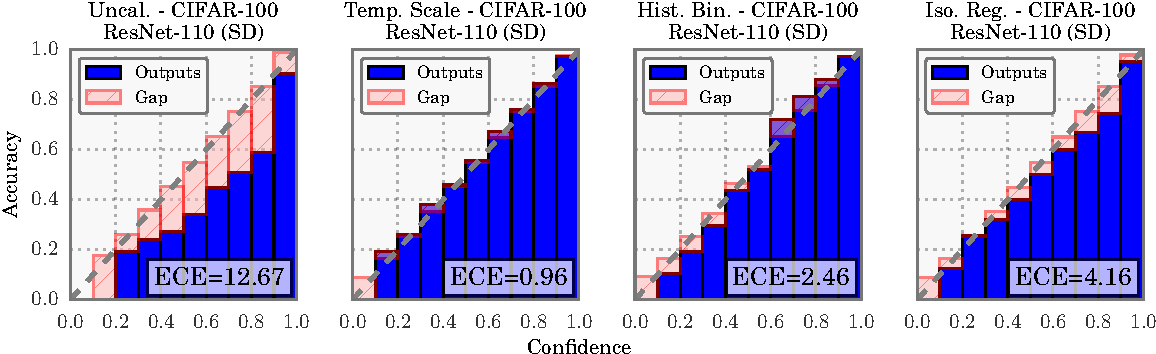
\includegraphics[width=0.98\textwidth]{fig/reliability-cifar100.pdf}
	\caption{Reliability diagrams for CIFAR-100 before (far left) and after calibration (middle left, middle right, far right).}
	\label{figure.reliability}
\end{figure*}

\paragraph{Calibration Results.}
\autoref{table.ece} displays model calibration, as measured by ECE (with $M=15$ bins), before and after applying the various methods (see \autoref{sup:tables} for MCE, NLL, and error tables).
It is worth noting that most datasets and models experience some degree of miscalibration, with ECE typically between $4$ to $10\%$.
This is not architecture specific: we observe miscalibration on convolutional networks (with and without skip connections), recurrent networks, and deep averaging networks.
 % problem problem of miscalibration is very pronounced on these recurrent neural networks. This is consistent with our observation that deeper networks tend to be less calibrated, as RNNs can be understood as extremely deep feed-forward networks~\cite{hochreiter1997long}.
The two notable exceptions are SVHN and Reuters, both of which experience ECE values below $1\%$. Both of these datasets have very low error ($1.98\%$ and $2.97\%$, respectively); and therefore the ratio of ECE to error is comparable to other datasets.

Our most important discovery is the \emph{surprising effectiveness of temperature scaling} despite its remarkable simplicity. Temperature scaling outperforms all other methods on the vision tasks, and performs comparably to other methods on the NLP datasets. What is perhaps even more surprising is that temperature scaling outperforms the vector and matrix Platt scaling variants, which are strictly more general methods. In fact, vector scaling recovers essentially the same solution as temperature scaling -- the learned vector has nearly constant entries, and therefore is no different than a scalar transformation. In other words, network miscalibration is intrinsically low dimensional.

The only dataset that temperature scaling does not calibrate is the Reuters dataset. In this instance, only one of the above methods is able to improve calibration. Because this dataset is well-calibrated to begin with (ECE $\leq 1\%$), there is not much room for improvement with any method, and post-processing may not even be necessary to begin with. It is also possible that our measurements are affected by dataset split or by the particular binning scheme.

% However, on Reuters, vector scaling performs considerably better than temperature scaling. We suspect this is due to class imbalance, as the network becomes overconfident about different classes at different rates. We investigated into this phenomenon by weighting the NLL loss by the inverse of class proportions, i.e. $$\scrL_{\rho}(\mathbf{x},\mathbf{y}) = -\sum_{i=1}^{n} \frac{\log(\hat{\pi}(y_i|x_i))}{\rho^{(y_i)}}$$ where $\rho^{(k)}$ is the proportion of class $k$ in the training set. By artificially balancing the classes this way, we find that temperature scaling performs similarly to vector scaling and the optimal scaling vector has equal entries once again.

Matrix scaling performs poorly on datasets with hundreds of classes (i.e. Birds, Cars, and CIFAR-100), and fails to converge on the 1000-class ImageNet dataset.
This is expected, since the number of parameters scales quadratically with the number of classes.
Any calibration model with tens of thousands (or more) parameters will overfit to a small validation set, even when applying regularization.

Binning methods improve calibration on most datasets, but do not outperform temperature scaling. Additionally, binning methods tend to change class predictions which hurts accuracy (see \autoref{sup:tables}). Histogram binning, the simplest binning method, typically outperforms isotonic regression and BBQ, despite the fact that both methods are strictly more general. This further supports our finding that calibration is best corrected by simple models.

\paragraph{Reliability diagrams.} \autoref{figure.reliability} contains reliability diagrams for 110-layer ResNets on CIFAR-100 before and after calibration. From the far left diagram, we see that the uncalibrated ResNet tends to be overconfident in its predictions. We then can observe the effects of temperature scaling (middle left), histogram binning (middle right), and isotonic regression (far right) on calibration. All three displayed methods produce much better confidence estimates. Of the three methods, temperature scaling most closely recovers the desired diagonal function. Each of the bins are well calibrated, which is remarkable given that all the probabilities were modified by only a single parameter. We include reliability diagrams for other datasets in \autoref{sup:reliability}.

\paragraph{Computation time.} All methods scale linearly with the number of validation set samples. Temperature scaling is by far the fastest method, as it amounts to a one-dimensional convex optimization problem. Using a conjugate gradient solver, the optimal temperature can be found in 10 iterations, or a fraction of a second on most modern hardware. In fact, even a naive line-search for the optimal temperature is faster than any of the other methods. The computational complexity of vector and matrix scaling are linear and quadratic respectively in the number of classes, reflecting the number of parameters in each method. For CIFAR-100 ($K=100$), finding a near-optimal vector scaling solution with conjugate gradient descent requires at least 2 orders of magnitude more time. Histogram binning and isotonic regression take an order of magnitude longer than temperature scaling, and BBQ takes roughly 3 orders of magnitude more time.

\paragraph{Ease of implementation.} BBQ is arguably the most difficult to implement, as it requires implementing a model averaging scheme.
While all other methods are relatively easy to implement, temperature scaling may arguably be the most straightforward to incorporate into a neural network pipeline.
In Torch7 \citep{collobert2011torch7}, for example, we implement temperature scaling by inserting a \texttt{nn.MulConstant} between the logits and the softmax, whose parameter is $1/T$.
We set $T\!=\!1$ during training, and subsequently find its optimal value on the validation set.\footnote{
  For an example implementation, see \url{http://github.com/gpleiss/temperature_scaling}.
}

%% !TeX root = ../main.tex

%\item The validation set NLL never increases, which means that there can be no harm done.
%\item The entire process takes almost no computation or implementation effort compared to network training.
%\item Sec.\ref{results} empirically demonstrates our effectiveness on various state-of-the-art neural network models. We obtain much better NLL and calibration than the baselines introduced in Sec.\ref{related}, and even the model left of the gap.
% with the best validation NLL.
%\end{enumerate}
%Before going into the empirical results, we next offer two new perspectives on why our method could work well. Through our analysis, we also hope to bring more insights to neural network training in general.

Modern neural networks exhibit a strange phenomenon: probabilistic error and miscalibration worsen even as classification error is reduced.
We have demonstrated that recent advances in neural network architecture and training -- model capacity, normalization, and regularization -- have strong effects on network calibration.
It remains future work to understand why these trends affect calibration while improving accuracy.
Nevertheless, simple techniques can effectively remedy the miscalibration phenomenon in neural networks.
Temperature scaling is the simplest, fastest, and most straightforward of the methods, and surprisingly is often the most effective.
% We hope that the simplicity of this approach enables practitioners to easily produce well-calibrated neural networks.

\chapter{Detecting Neural Network Out-of-Distribution Inputs for Regression.}

\chapter{Simplifying and Scaling Gaussian Process Training with Blackbox Matrix-Matrix Inference}

\chapter{Speeding up Gaussian Process Predictions with Lanczos Variance Estimates}

\chapter{Conclusion and Future Directions}
\label{chapter:discussion}


This thesis has presented a comprehensive framework for Gaussian process training, inference, and prediction.
The algorithms proposed in \cref{chapter:bbmm,chapter:love,chapter:ciq} are based around a single central design decision: reduce all expensive matrix operations to parallelized matrix-vector multiplications (MVMs).
\cref{chapter:bbmm} introduced the Black-Box Matrix~\texttimes~Matrix (BBMM) framework which computes GP training terms via a modified batched-conjugate gradients algorithm (mBCG).
To enable fast predictions with GP models, \cref{chapter:love} presented LanczOs Variance Estimates (LOVE), which computes an amortized cache of the predictive posterior.
Finally, \cref{chapter:ciq} introduced Cauchy Integral Quadrature (CIQ) to ``whiten'' and ``unwhiten'' vectors with respect to a Gaussian covariance---enabling
the MVM-based training of variational GP models and also allowing efficient posterior sampling.

The MVM theme simultaneously addresses several desiderata for Gaussian processes.
As demonstrated in \cref{chapter:bbmm}, MVM-based methods effectively utilize GPU hardware and reduce specialty implementations to $\leq 50$ lines of code.
This makes it easy for researchers to rapidly prototype and test novel models across a wide variety of datasets.
%MVM-based methods also reduce the asymptotic complexity of GPs, which in turn allows for in more powerful predictions and inferences.
MVM-based methods also lead to faster, more powerful models.
\cref{chapter:love} significantly reduces computational costs of GPs at test-time, while
\cref{chapter:ciq} scales up variational approximations and large-scale sampling, leading to better predictions and black-box optimization.
Combined, these methods expand what is considered tractable for exact GPs, as demonstrated in the $N=1,\!000,\!000$ experiments of \cref{chapter:largeexact}.
\clearpage



\section{Beyond Matrix-Vector Multiplication}

The framework presented in this thesis makes GPs increasingly practical on massive datasets.
%Moreover, standard GP models can be an effective model class for many large datasets (as demonstrated in \cref{sec:largeexact_results}).
Large-scale problems allow for more powerful classes of GP-based models, which in turn opens up many exciting research problems.
%These problems go beyond the scope of what is addressed by the MVM methods in this thesis.

To increase the representational capacity of Gaussian processes, researchers have proposed highly-parametric kernels \cite{wilson2013gaussian,wilson2016stochastic}, using GPs as components of larger pipelines \cite{schulam2015framework,futoma2017learning}, and hierarchical GP models \cite{wilson2012gaussian,salimbeni2017doubly,jankowiak2020deep}.
%These models are an attractive choice for large-scale modelling: combining the expressively and capacity of techniques like deep learning with the probabilistic capabilities afforded by Gaussian processes.
Of course, the additional complexity of these approaches may pose new training and inference challenges.
Advances in large-scale optimization have mostly targeted the piece-wise linear geometry of ReLU neural networks and may need to be adapted to the geometry of Gaussian processes-based models.
This is especially true for GP models that use alternative objective functions for learning \cite{sheth2017excess,knoblauch2019generalized,jankowiak2020parametric}.
Moreover, hierarchical GP models are more computationally intensive than simpler models.
%Deep Gaussian processes for example stack multiple GPs on top of one another, and BBMM-style methods should be adapted to handle this sequential computation.
Such models necessitate parametric approximations, as exact inference is intractable.
Consequentially, increasing the fidelity of these models (e.g. stacking more layers, using more inducing points) increases the number of parameters, which may become an optimization or test-time bottleneck.
It is worth noting that these problems are not unique to large-scale Gaussian processes---they are also issues of other large-scale machine learning models.
Addressing these challenges in the context of GPs however is a relatively new area of research, as these models have only recently been considered practical.




\section{Beyond Gaussian Processes}

A key insight of this thesis is that non-linear operations on large-scale kernel matrices are surprisingly tractable when used in conjunction with GPU acceleration and efficient numerical techniques.
While we motivate this finding through GPs, it is worth noting that the algorithms presented here are applicable to other classes of models.
For example, a common relaxation to optimal transport problems is solved via Sinkhorn iterations \cite{cuturi2013sinkhorn}, which rely on iterative MVMs with an exponentiated distance matrix.
%This exponentiated distance matrix can be interpreted as a scaled RBF kernel, and therefore the preconditioning and partitioning techniques from this thesis might scale this algorithm beyond its current limits.
Second-order optimization is another application where large-scale solves are necessary.
GPU-accelerated MVM methods may make such methods applicable to higher dimensional problems \cite{koh2017understanding}.

More generally, machine learning in recent years has shied away from complex matrix operations.
Many modern algorithms instead derive expressive power through the composition of linear and element-wise functions \cite{goodfellow2016deep}.
While deep neural networks demonstrate the merit of this approach, it is possible that incorporating more complex matrix operations could improve parameter efficiency and model capacity \cite{jankowiak2020deep}.
The ability to efficiently compute arbitrary functions of big matrices opens up possibilities well beyond large-scale Gaussian process models.



\appendix

\bibliography{gpleiss_thesis}
\end{document}
